\section{DFDS}
A data flow diagram (DFD) is a graphical representation of the "flow" of data through an information system, modelling its process aspects. A DFD is often used as a preliminary step to create an overview of the system, which can later be elaborated.	DFDs of DoS is as following-: 
\begin{figure}[H]
\centering 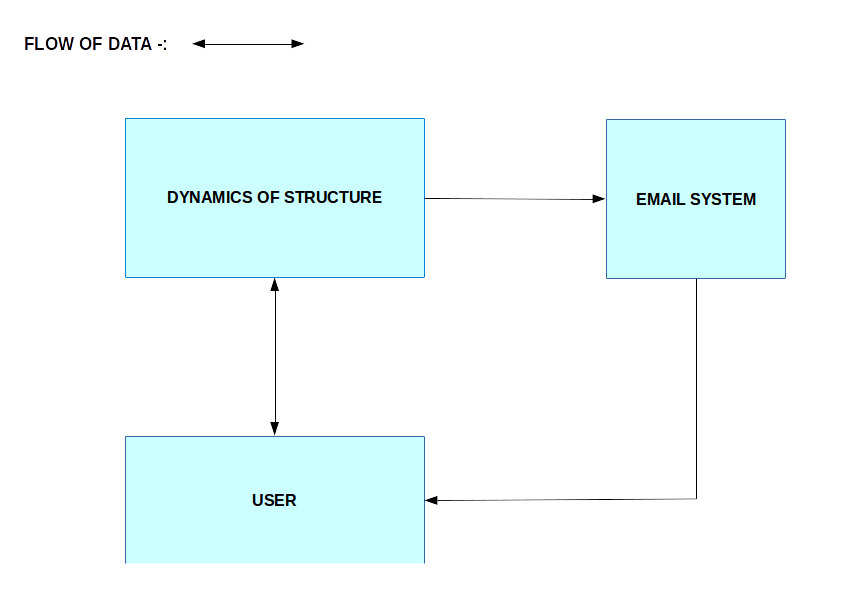
\includegraphics[scale=0.4]{images/DFDS.png}
\caption{Data flow LEVEL 0}
\end{figure}
\begin{figure}[H]
\centering 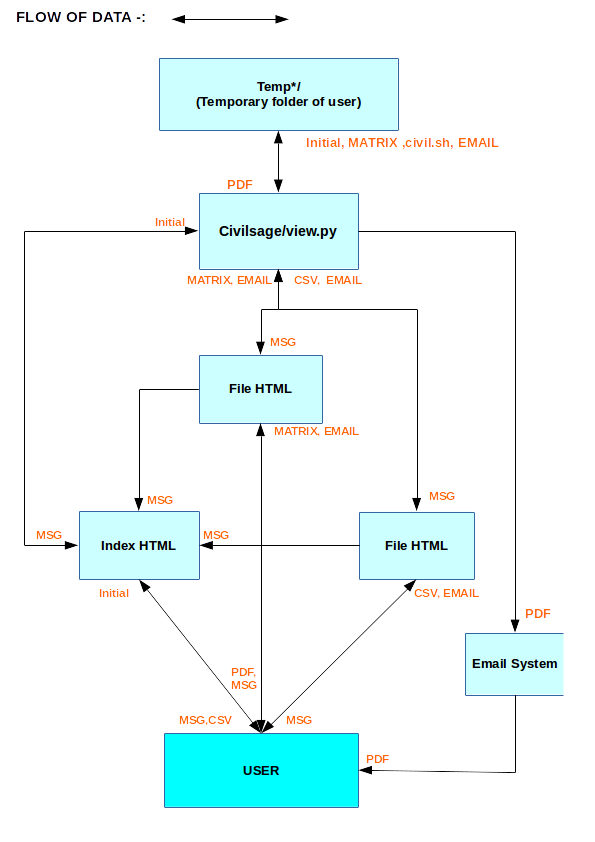
\includegraphics[scale=0.55]{images/DFDS1.png}
\caption{Data Flow LEVEL 1}
\end{figure}
\section{UI Flow Diagram}
UI Flow diagram tells how user will precive different interface on click of different buttons or trigger and UI flow Diagram of DoS is given below-: 
\begin{figure}[H]
\centering 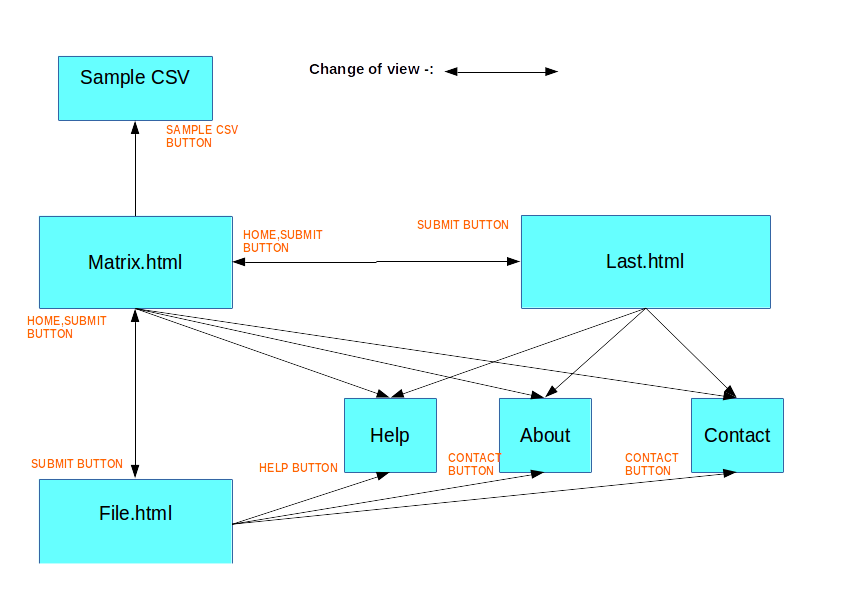
\includegraphics[scale=0.55]{images/UI.png}
\caption{UI Flow diagram}
\end{figure}
\section{Flowchart}
A flowchart is a type of diagram that represents an algorithm, workflow or process, showing the steps as boxes of various kinds, and their order by connecting them with arrows
and following are flowchart of DoS showing flow of control and Data in the software-:

\begin{figure}[H]
\centering 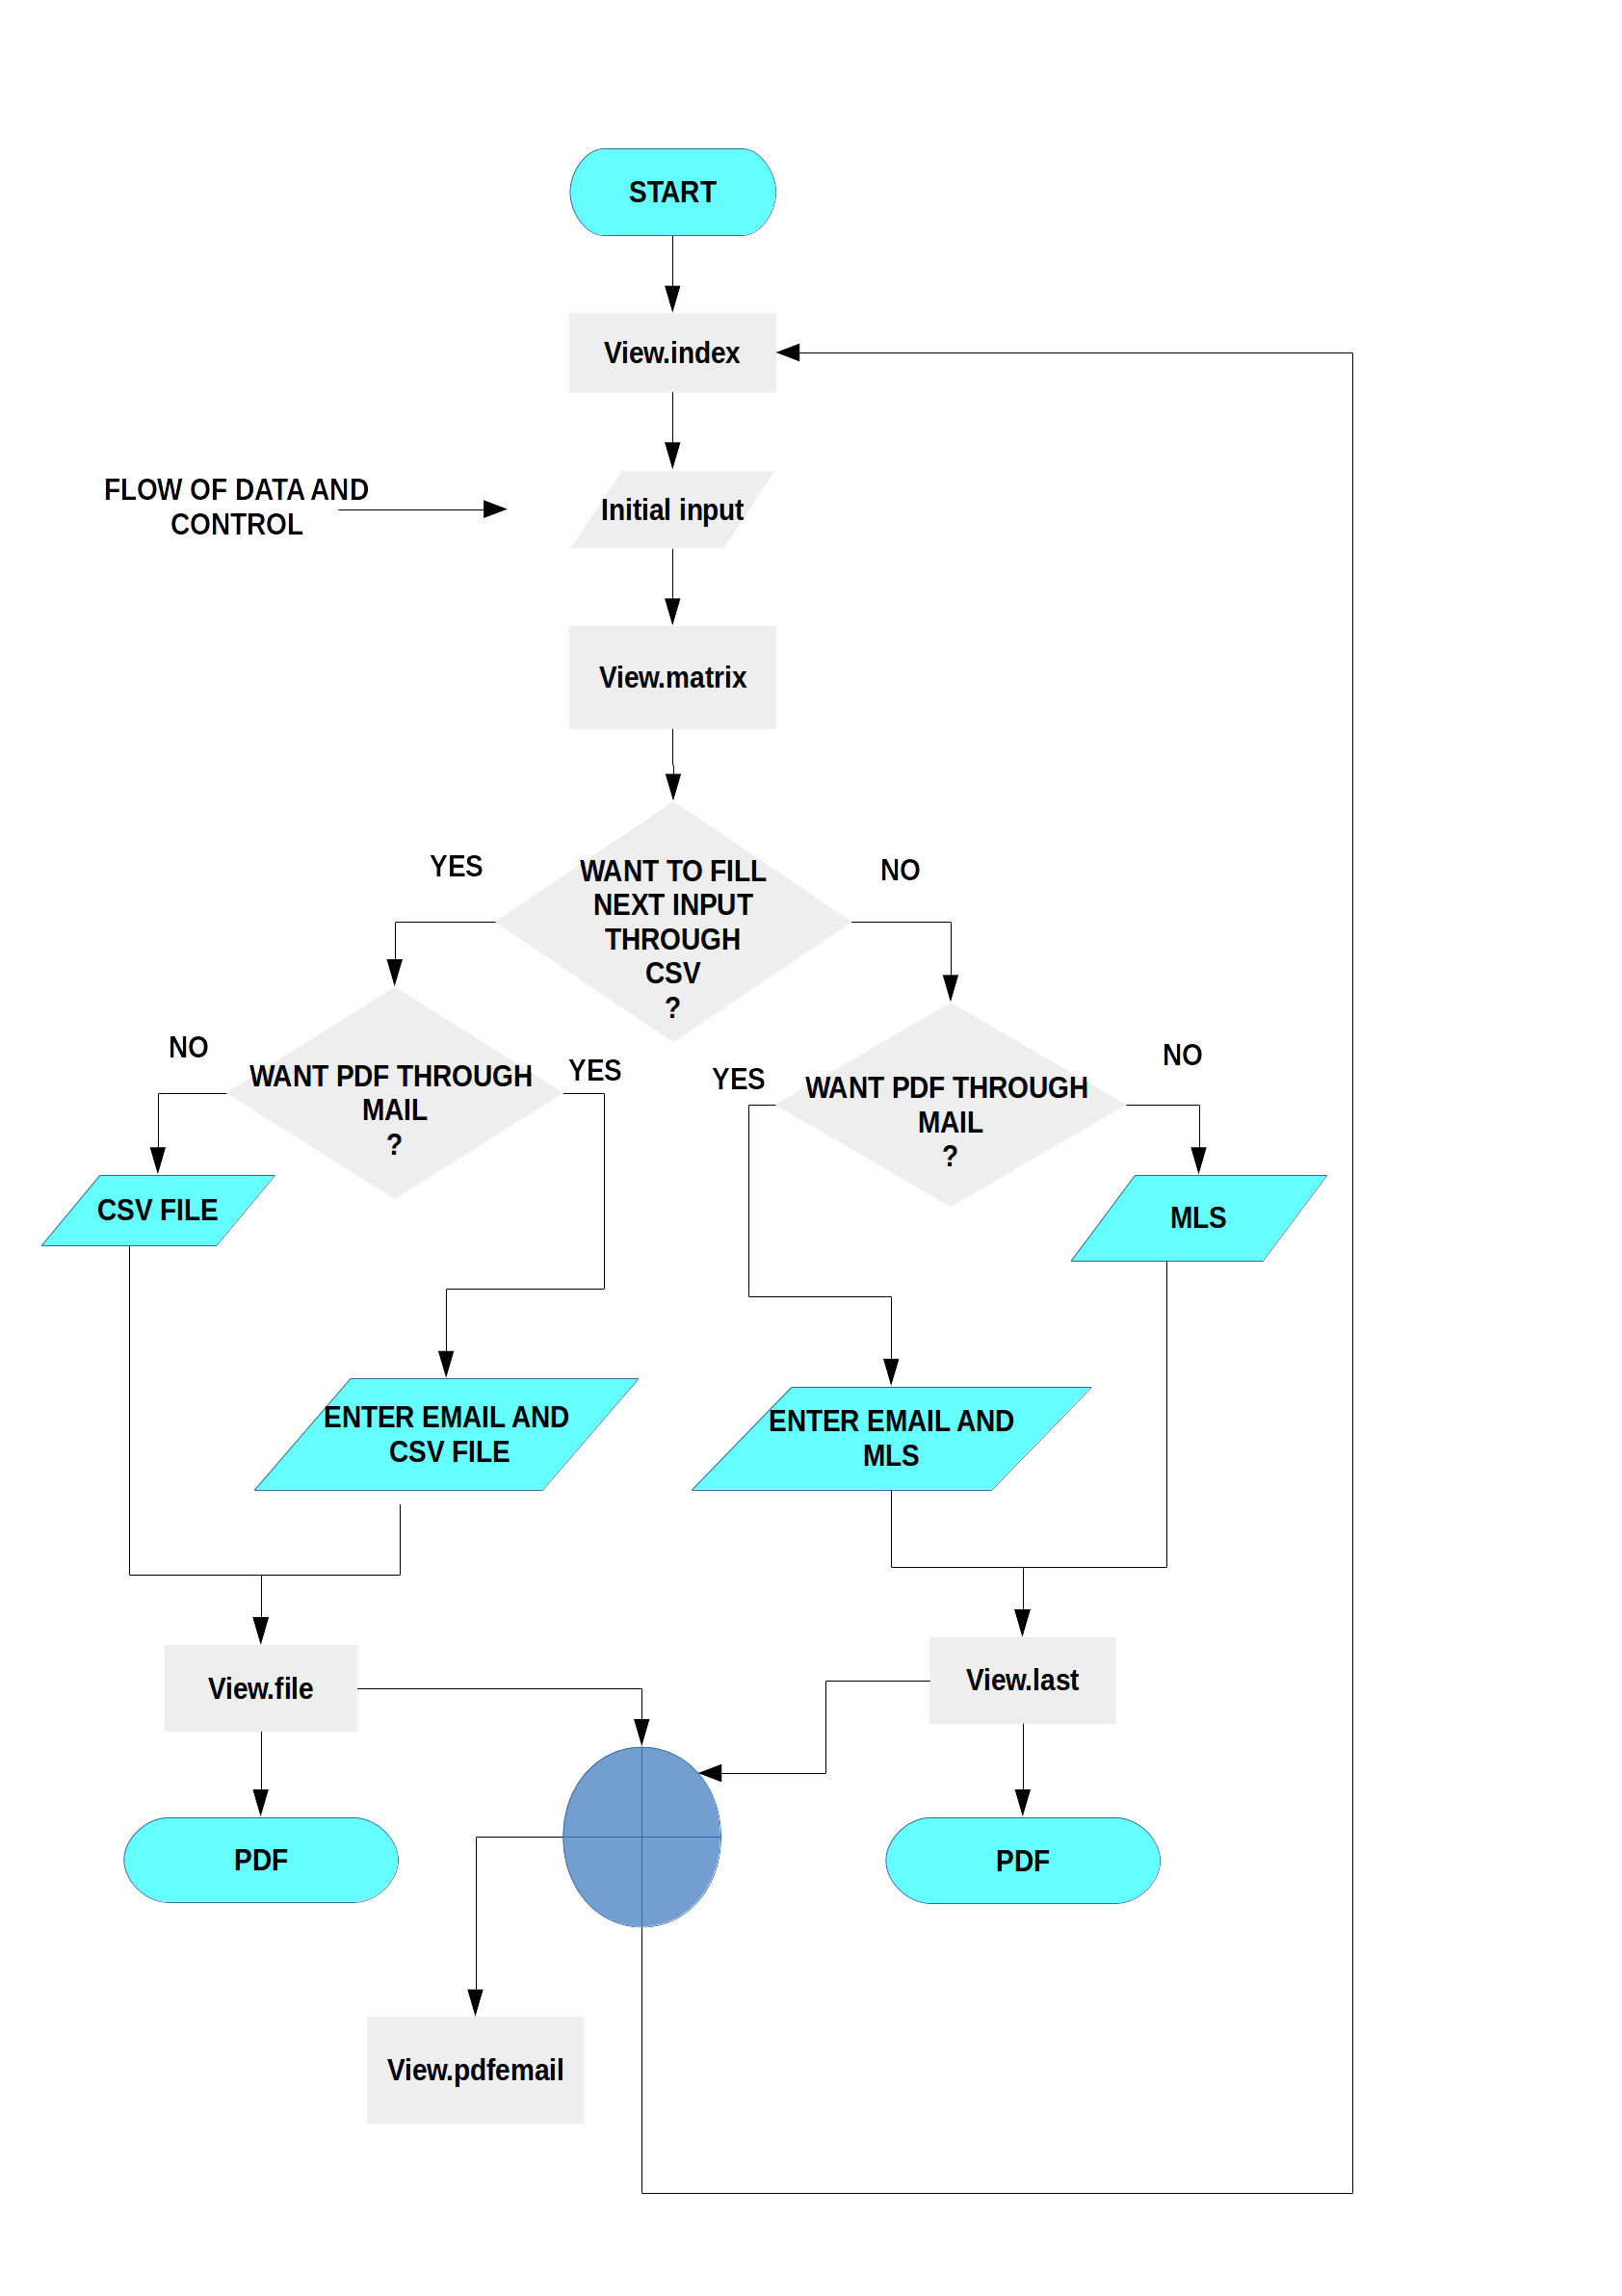
\includegraphics[scale=0.26]{images/flowchart.png}
\caption{Flowchart of Whole System}
\end{figure}
\begin{figure}[H]
\centering 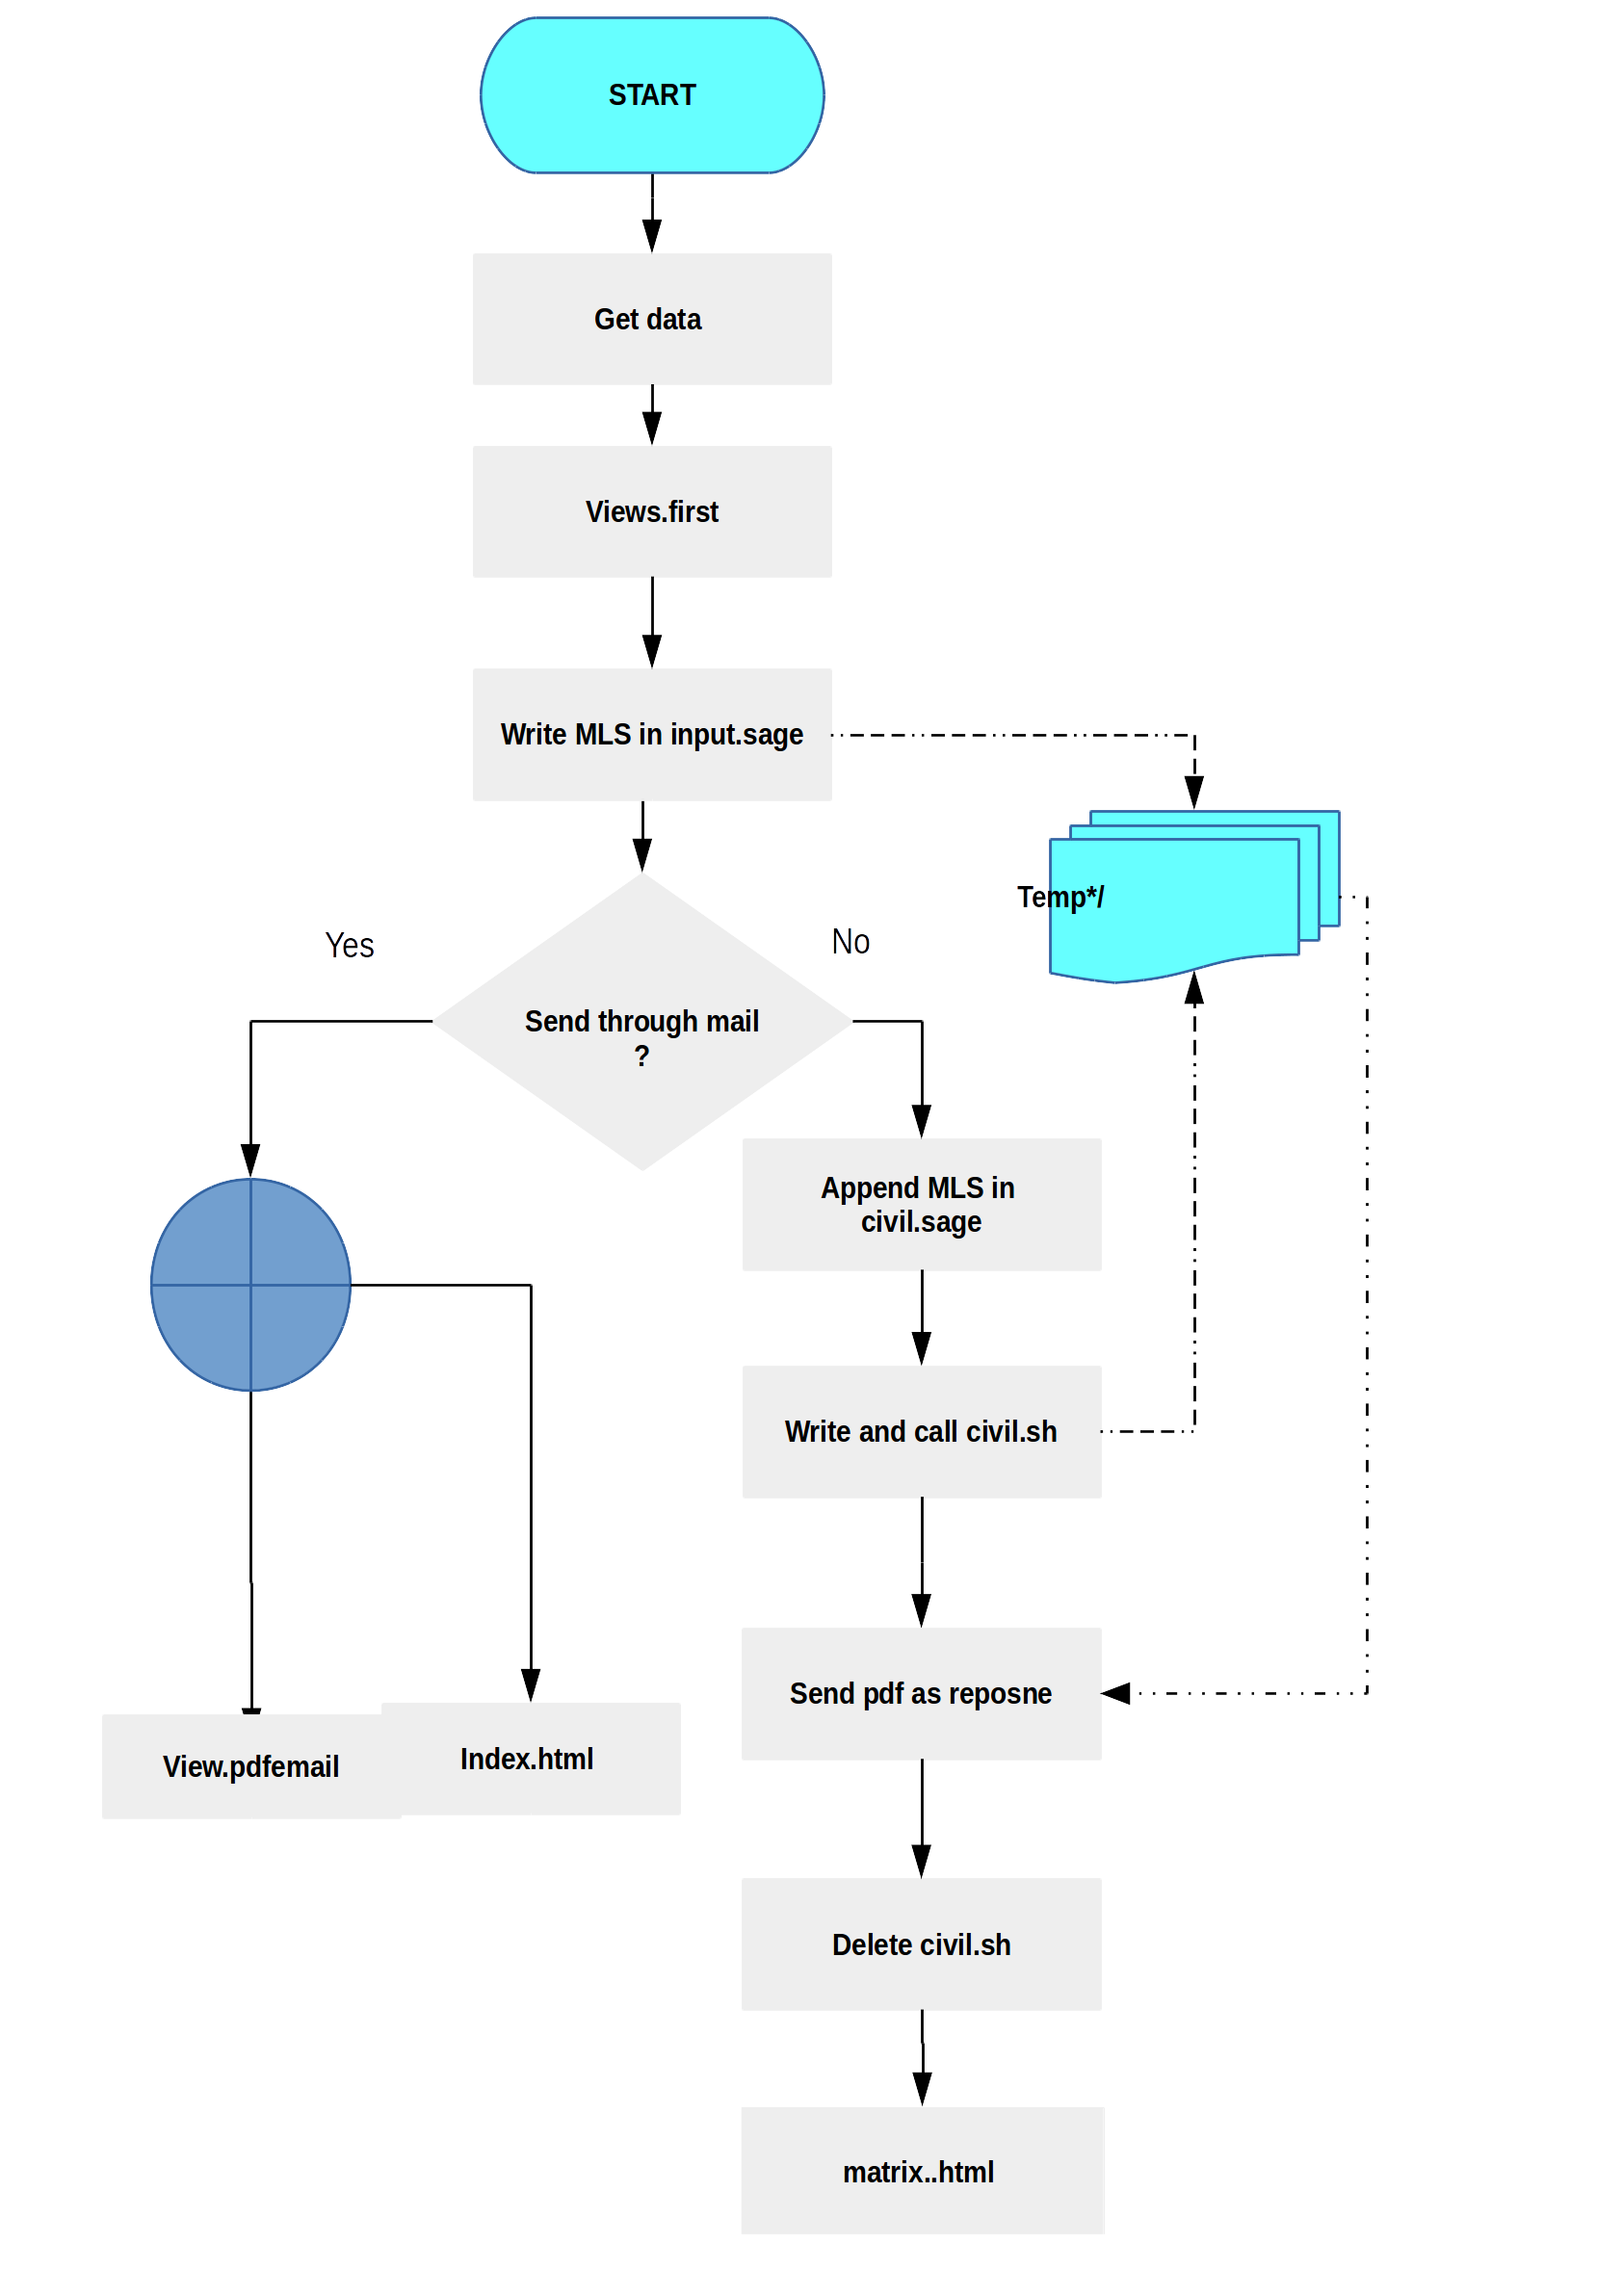
\includegraphics[scale=0.27]{images/flowchartmatrix.png}
\caption{Flowchart of veiw.matrix}
\end{figure}
\begin{figure}[H]
\centering 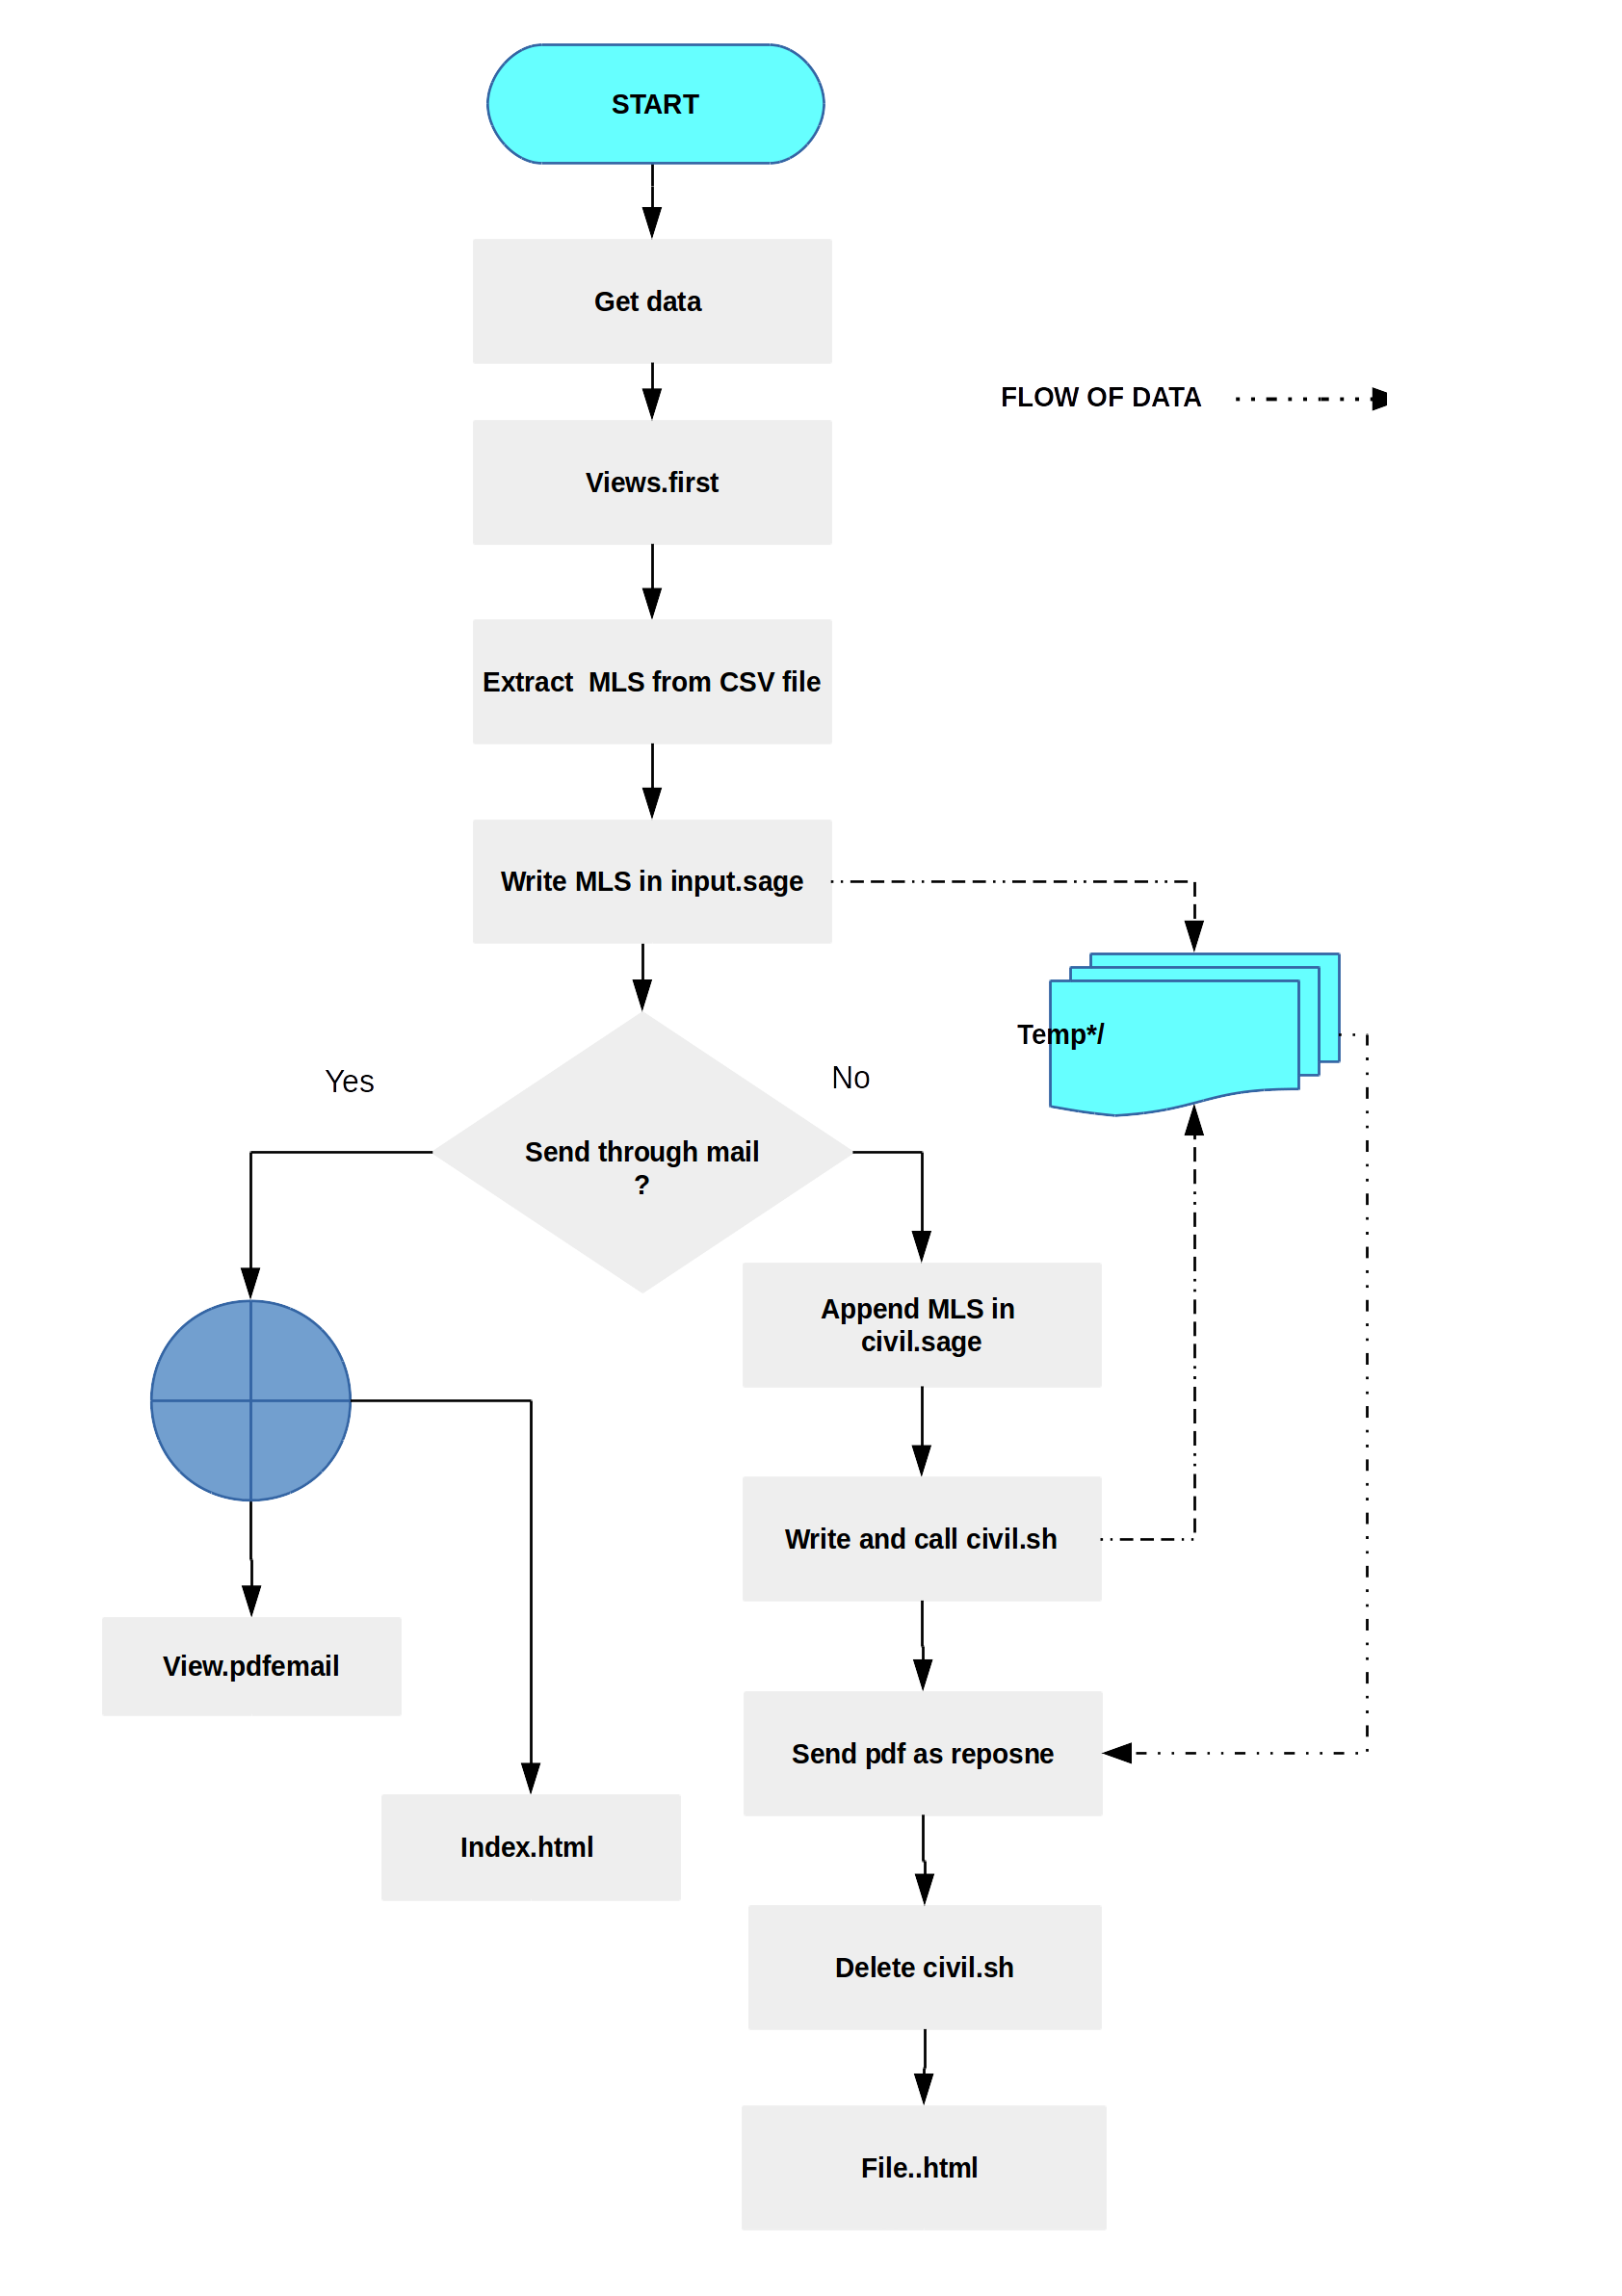
\includegraphics[scale=0.27]{images/flowchartfile.png}
\caption{Flowchart of veiw.file}
\end{figure}
\begin{figure}[H]
\centering 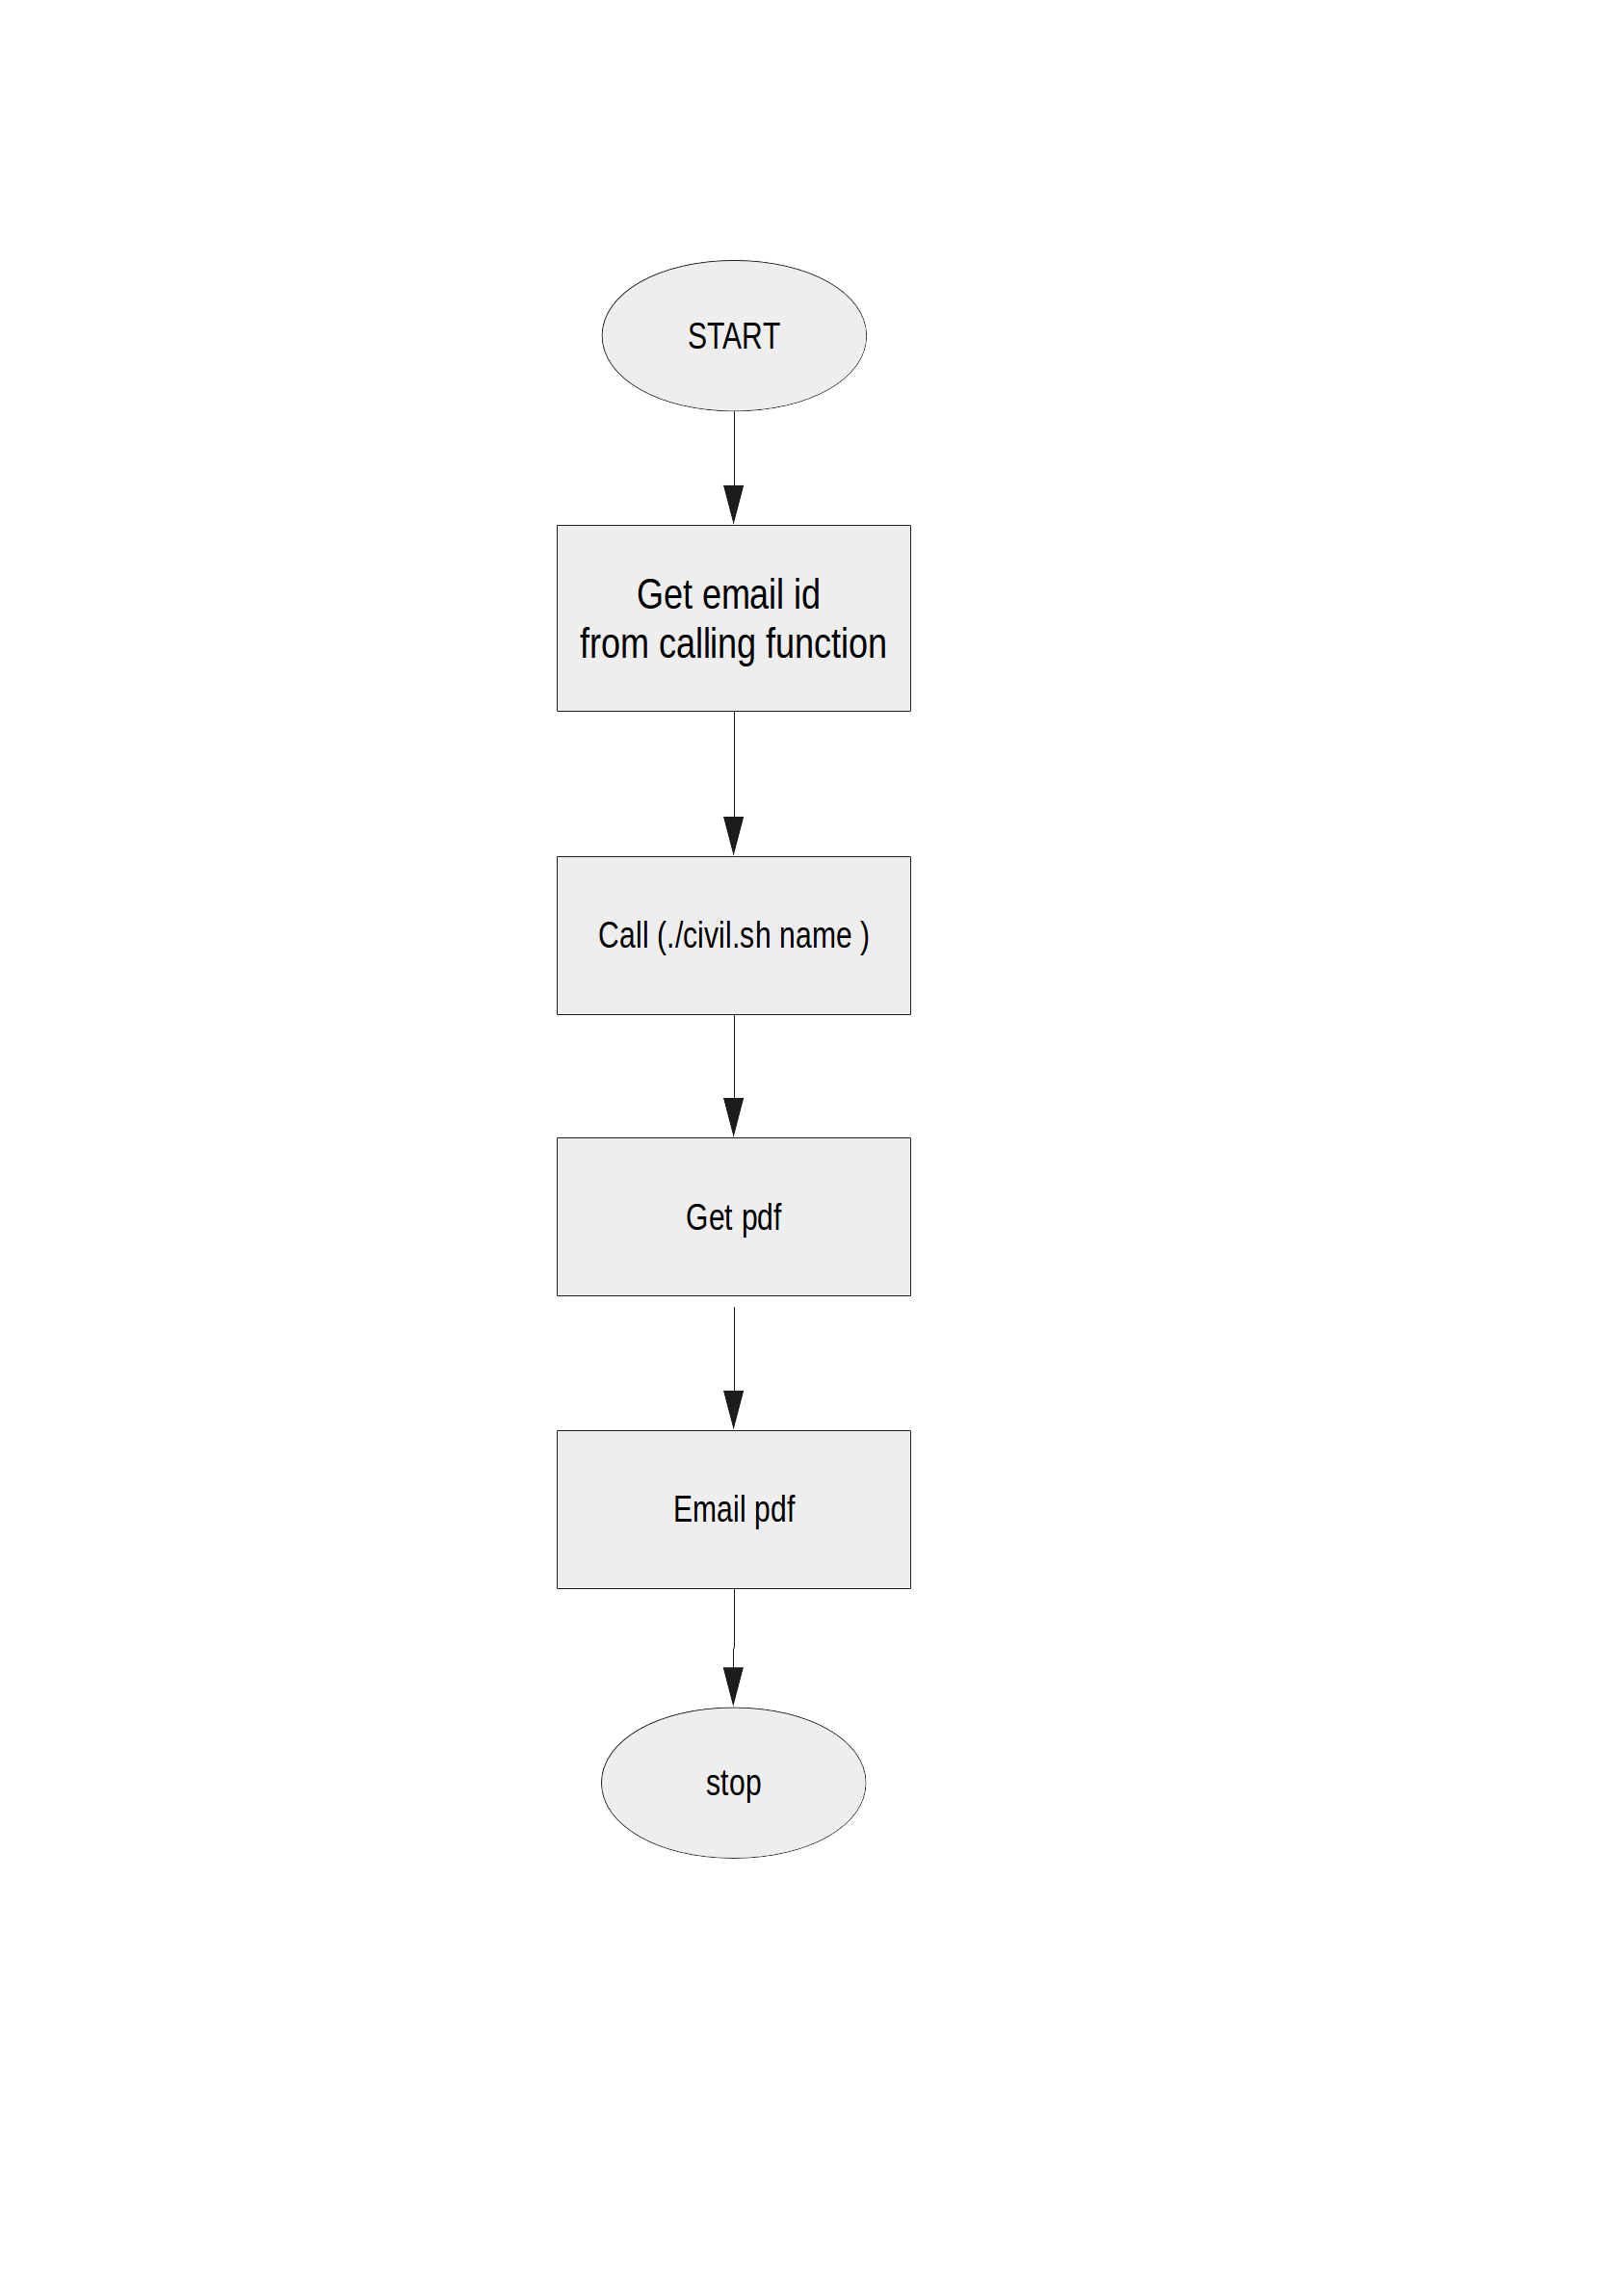
\includegraphics[scale=0.27]{images/flowchartpdf.png}
\caption{Flowchart of veiw.pdfemail}
\end{figure}
\begin{figure}[H]
\centering 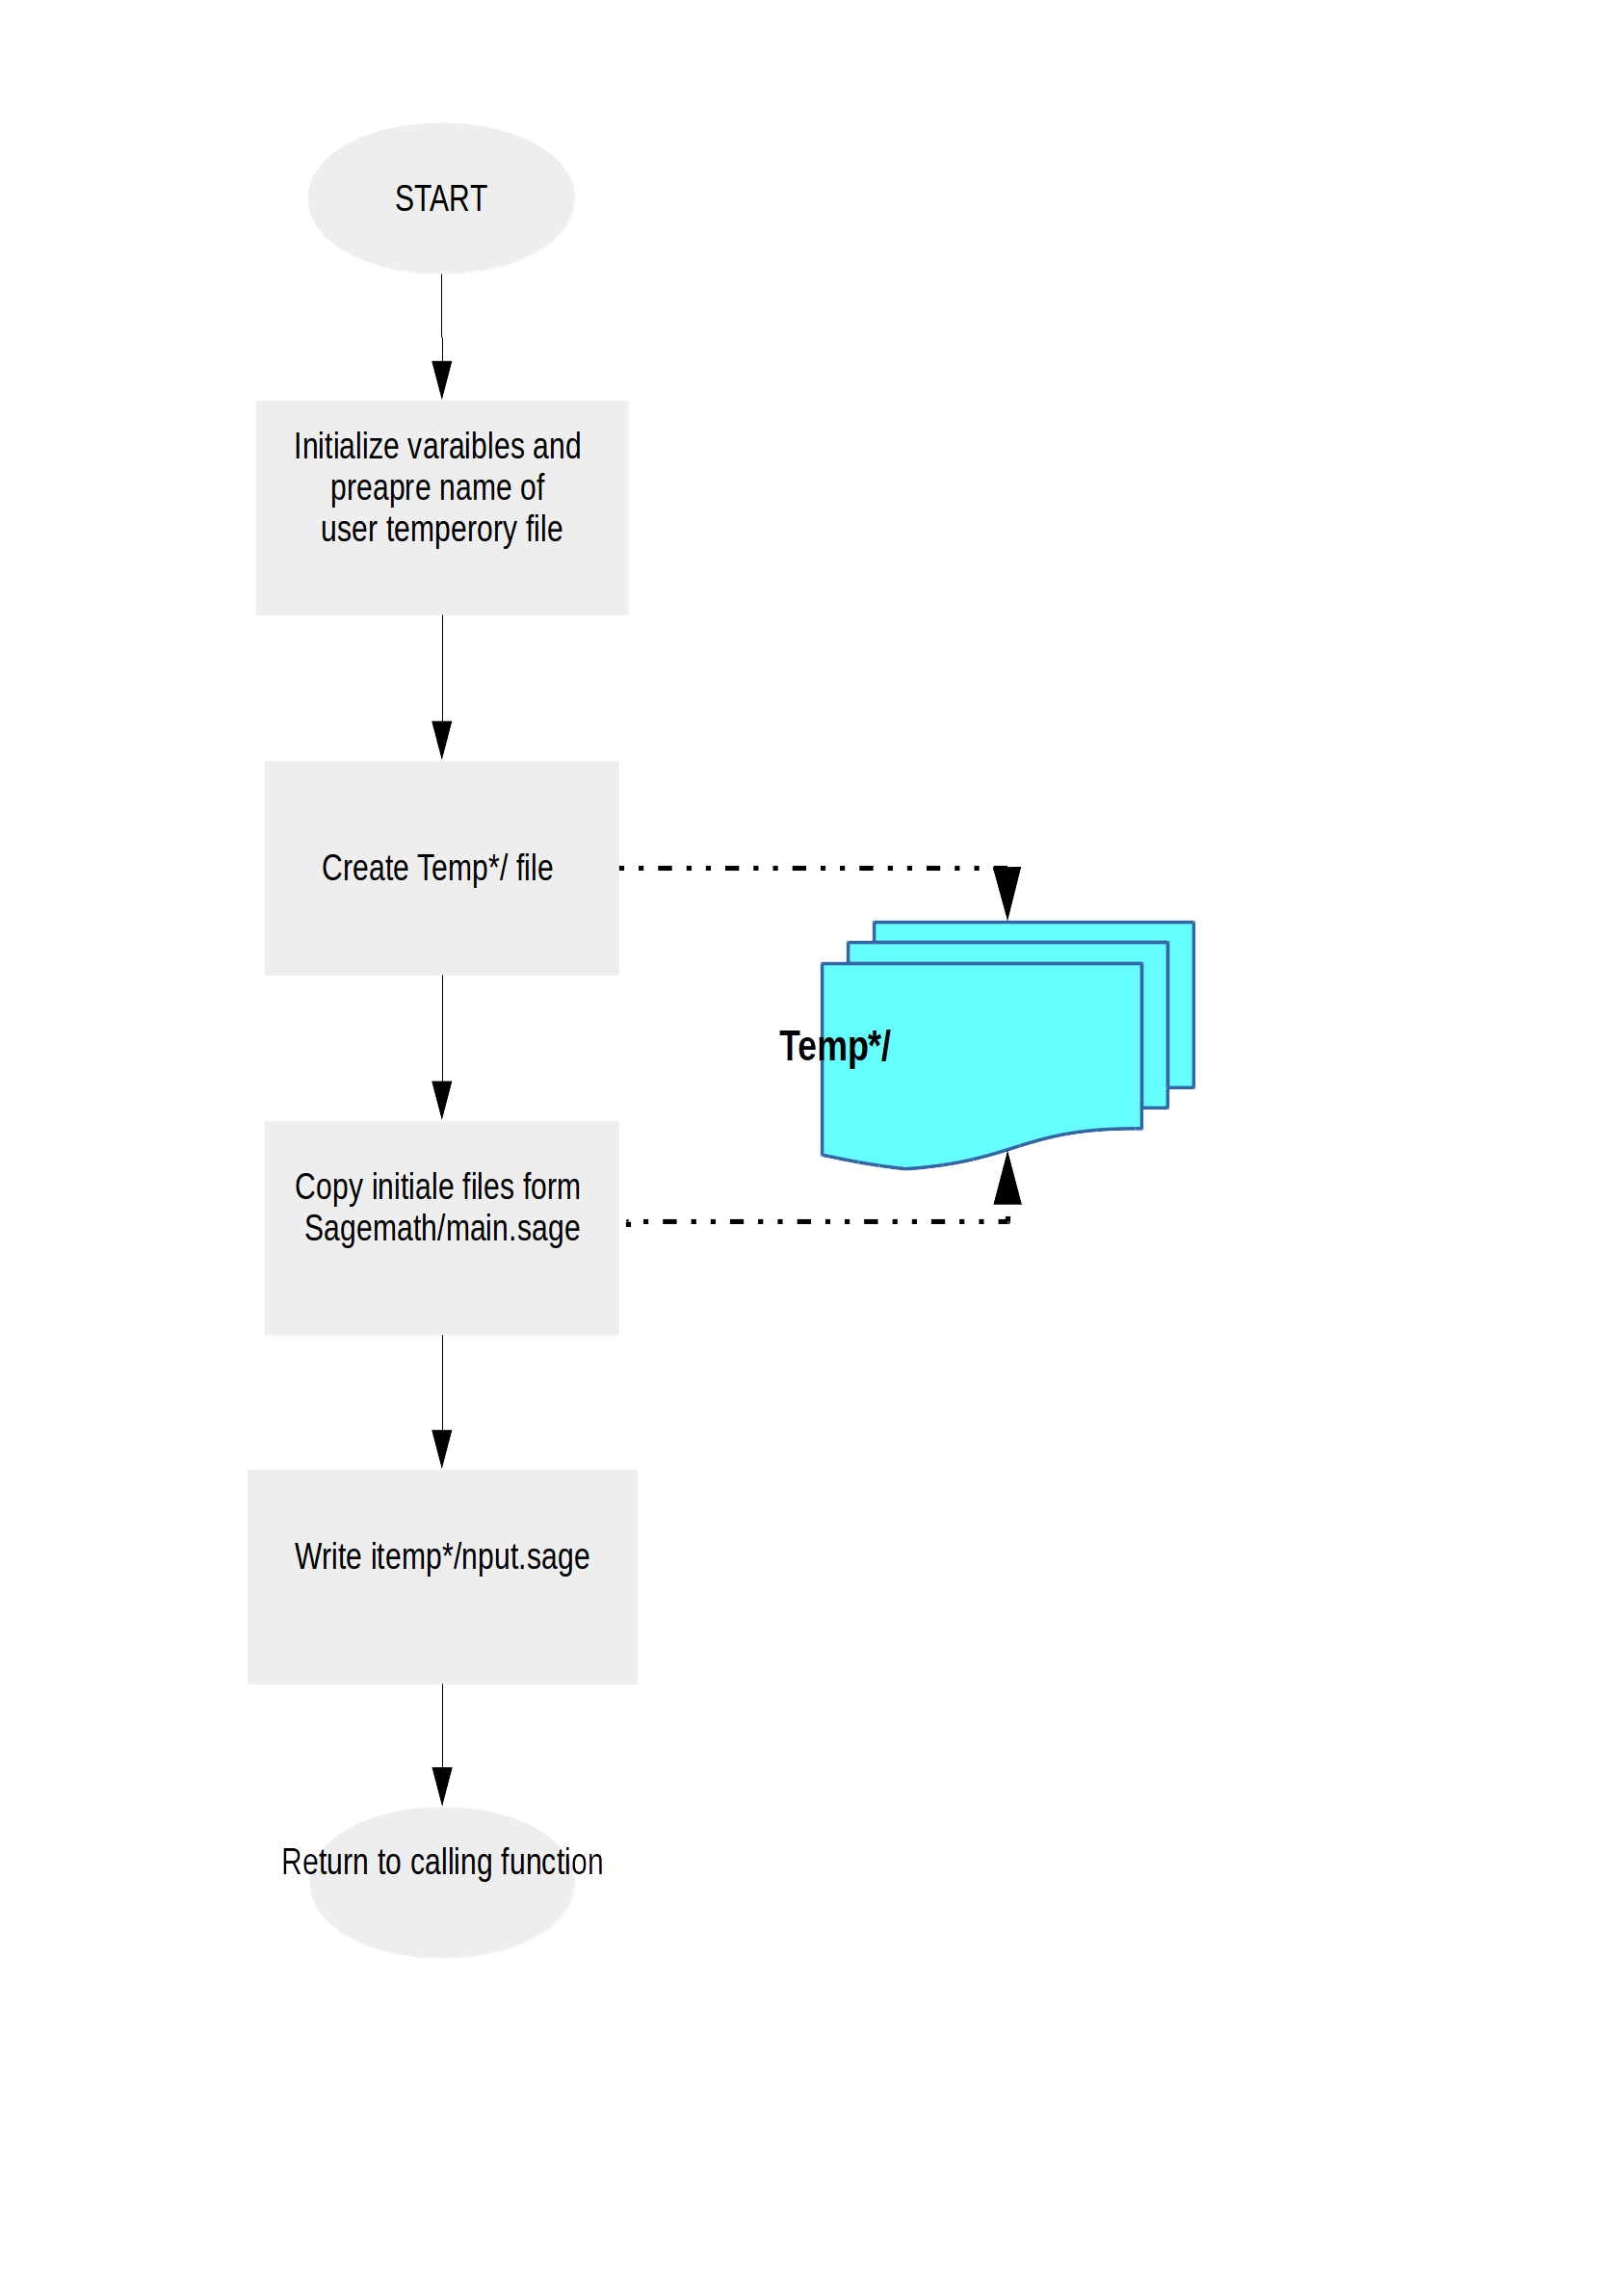
\includegraphics[scale=0.27]{images/flowchartfirst.png}
\caption{Flowchart of veiw.first}
\end{figure}

